%%%%%%%%%%%%%%%%%%%%%%%%%%%%%%%%%%%%%%%%%%%%%%%%%
% This tex file uses minted package.
% Do not compile if Pygments highlighter for 
% minted is not installed. 
% Use admin to compile this file.
% External data file is provided in the alg/ folder.
%%%%%%%%%%%%%%%%%%%%%%%%%%%%%%%%%%%%%%%%%%%%%%%%%

\documentclass[12pt,a4paper]{article}
\usepackage{amsmath,amscd,amsbsy,amssymb,latexsym,url,bm,amsthm}
\usepackage{epsfig,graphicx,subfigure}
\usepackage{enumitem,balance}
\usepackage{wrapfig}
\usepackage{mathrsfs,euscript}
\usepackage[usenames]{xcolor}
\usepackage{hyperref}
\usepackage{booktabs}
\usepackage[vlined,ruled,linesnumbered]{algorithm2e}
\usepackage{threeparttable}
\hypersetup{colorlinks=true,linkcolor=black}

\newtheorem{theorem}{Theorem}
\newtheorem{lemma}[theorem]{Lemma}
\newtheorem{proposition}[theorem]{Proposition}
\newtheorem{corollary}[theorem]{Corollary}
\newtheorem{exercise}{Exercise}
\newtheorem*{solution}{Solution}
\newtheorem{definition}{Definition}
\theoremstyle{definition}

\renewcommand{\thefootnote}{\fnsymbol{footnote}}

\newcommand{\postscript}[2]
 {\setlength{\epsfxsize}{#2\hsize}
  \centerline{\epsfbox{#1}}}

\renewcommand{\baselinestretch}{1.0}

\setlength{\oddsidemargin}{-0.365in}
\setlength{\evensidemargin}{-0.365in}
\setlength{\topmargin}{-0.3in}
\setlength{\headheight}{0in}
\setlength{\headsep}{0in}
\setlength{\textheight}{10.1in}
\setlength{\textwidth}{7in}
\makeatletter \renewenvironment{proof}[1][Proof] {\par\pushQED{\qed}\normalfont\topsep6\p@\@plus6\p@\relax\trivlist\item[\hskip\labelsep\bfseries#1\@addpunct{.}]\ignorespaces}{\popQED\endtrivlist\@endpefalse} \makeatother
\makeatletter
\renewenvironment{solution}[1][Solution] {\par\pushQED{\qed}\normalfont\topsep6\p@\@plus6\p@\relax\trivlist\item[\hskip\labelsep\bfseries#1\@addpunct{.}]\ignorespaces}{\popQED\endtrivlist\@endpefalse} \makeatother

\providecommand{\limn}{\lim_{n\rightarrow \infty}}
\usepackage{tikz}
\usepackage{pgfplots}
\pgfplotsset{compat=1.14}
\usepgfplotslibrary{colorbrewer}
\usepackage{codeblock}
\usepackage{multicol}

\begin{document}
\noindent

%========================================================================
\noindent\framebox[\linewidth]{\shortstack[c]{
\Large{\textbf{Lab01-Algorithm Analysis}}\vspace{1mm}\\
CS214-Algorithm and Complexity, Xiaofeng Gao, Spring 2021.}}
\begin{center}
\footnotesize{\color{red}$*$ If there is any problem, please contact TA Haolin Zhou. Also please use English in homework.}

% Please write down your name, student id and email.
\footnotesize{\color{blue}$*$ Name: Log Creative  \quad Student ID:  \quad Email: logcreative-lzl@sjtu.edu.cn}
\end{center}

\begin{enumerate}


\item \textit{Complexity Analysis.} Please analyze the time and space complexity of Alg.~\ref{Alg-quicksort} and Alg.~\ref{Alg-cocktailsort}. \par

\begin{minipage}[t]{0.45\textwidth}
	\begin{algorithm}[H]
		\KwIn{An array $A[1,\cdots,n]$}
		\KwOut{$A[1,\cdots,n]$ sorted nondecreasingly}
		
		\BlankLine
		\caption{QuickSort}\label{Alg-quicksort}
		
		%\If{$n \le 1$}{
		%  \Return\;
		%}
		
		$pivot \leftarrow A[n]$; $i \leftarrow 1$\;
		\For{$j \leftarrow 1$ \KwTo $n-1$}{
			\If{$A[j] < pivot$}{
				swap $A[i]$ and $A[j]$\;
				$i \leftarrow i+1$\;
			}
		}
		
		swap $A[i]$ and $A[n]$\;
		\lIf{$i>1$}{$\operatorname{QuickSort}(A[1,\cdots,i-1])$}
		\lIf{$i<n$}{$\operatorname{QuickSort}(A[i+1,\cdots,n])$}
	\end{algorithm}
\end{minipage}
\hfill
\begin{minipage}[t]{0.45\textwidth}
\begin{algorithm}[H]
\KwIn{An array $A[1,\cdots,n]$}
\KwOut{$A[1,\cdots,n]$ sorted nonincreasingly}
\BlankLine
\caption{CocktailSort}
\label{Alg-cocktailsort}
\BlankLine
	$i\leftarrow 1;$ $j\leftarrow n;$$sorted\leftarrow false$\;
	\While{\textbf{not} sorted}{
		$sorted \leftarrow true$\;
		\For{$k\leftarrow i$ \textbf{to} $j-1$}{
			\If{$A[k] < A[k+1]$}{
				swap $A[k]$ and $A[k+1]$\;
				$sorted\leftarrow false$\;
			}
		}
		$j\leftarrow j-1$\;
		

		\For{$k\leftarrow j$ \textbf{downto} $i+1$}{
			\If{$A[k-1] < A[k]$}{
				swap $A[k-1]$ and $A[k]$\;
				$sorted\leftarrow false$\;
			}
		}
		$i\leftarrow i+1$\;
	}
\end{algorithm}
\end{minipage}

\begin{enumerate}
	 
\item Fill in the blanks and \textbf{explain} your answers. You need to answer when the best case and the worst case happen. 
\begin{table}[!h]

\label{Tab-compare}
	\centering
	\begin{threeparttable}
	\begin{tabular}{c|c| c }
		\toprule[2pt]
		\textbf{Algorithm} & \textbf{Time Complexity}\tnote{1} & \textbf{Space Complexity} \\
		\hline
		\hline
		$QuickSort$ & $\Omega(n\log n)$, $O(n \log n)$, $O(n^2)$ & $O(\log n)$ \\

		$CocktailSort$ & $\Omega(n)$, $O(n^2)$, $O(n^2)$ & $O(1)$  \\
		\bottomrule[2pt]


	\end{tabular}
    \begin{tablenotes}
    	\footnotesize
    	\item[1] The response order can be given in \emph{best}, \emph{average}, and \emph{worst}.
    \end{tablenotes}
	\end{threeparttable}
\end{table}

\item For Alg.~\ref{Alg-quicksort}, how to modify the algorithm to achieve the same expected performance as the \textbf{average} case when the \textbf{worst} case happens?
\end{enumerate} 
\begin{solution}
	\begin{enumerate}
		\item The problem only needs the proof of best and worst cases. So, I will not prove the conclusion of the average case. Instead, I will perform a series of test and note some thoughts to show that the conclusion is correct.
		
		Algorithm \ref{Alg-quicksort} -- QuickSort:
		\begin{description}
			\item[Best Case] $\Omega(n\log n)$ Appears when every time the pivot seperates the array into two equally-sized subarrays. Then the call could be a binary tree with approximately $\log n$ layers. In Layer $j$, there are $2^j$ partitions and $\frac{n}{2^j}$ elements every partition. Thus, the complexity comes to:
			\begin{equation*}
				T(n) \approx \sum_{j=1}^{\log n}\frac{n}{2^j}\times 2^j = n\log n = \Omega(n\log n)
			\end{equation*}
			
			\item[Worst Case] $O(n^2)$ Happens when every time the pivot always separates the array into 1 and $n-1$ sized subarrays. This may occur if the pivot happens to be the smallest element in every partition, for example, all the element are equal.

			Then, a linear chain of partitioning is produced and the time complexity comes to:
			\begin{equation*}
				T(n) = n + (n-1) + \cdots + 1 = \frac{(n+1)n}{2} = O(n^2)
			\end{equation*}

			\begin{minipage}[t]{0.4\textwidth}
				\begin{table}[H]
					\centering
					\begin{tabular}{ccc}
						\fbox{1} & 3 & \underline{2}\\
						1 & \underline{3} & \underline{2}\\
						1 & \fbox{3} & \fbox{2}\\
						\fbox{1} & 2 & 3\\
						1 & 2 & \fbox{3}\\
						1 & 2 & 3
					\end{tabular}	

					Best Case for QuickSort
				\end{table}
			\end{minipage}
			\begin{minipage}[t]{0.4\textwidth}
				\begin{table}[H]
					\centering
					\begin{tabular}{ccc}
						\underline{3} & 3 & \underline{3}\\
						3 & \underline{3} & \underline{3}\\
						\fbox{3} & 3 & \fbox{3}\\
						3 & \underline{3} & \underline{3}\\
						3 & \fbox{3} & \fbox{3}\\
						3 & 3 & \fbox{3}\\
						3 & 3 & 3
					\end{tabular}

					Worst Case for QuickSort
				\end{table}
			\end{minipage}

			\item[Average Case] $O(n\log n)$ The proof of the average case could be done by the master theorem for divide-and-conquer recurrences in the future.
			\item[Space Complexity] $O(\log n)$ The algorithm is done in place for every partition, which is $O(1)$ space, but the sort of every partition should be done recursively before the other in the same layer could be performed. Thus the call stack depth is bounded by $O(\log n)$ spaces.
		\end{description}
		% Todo: Space
		Algorithm \ref{Alg-cocktailsort} -- CocktailSort:
		\begin{description}
			\item[Best Case] $\Omega(n)$ Appears when the array has already been sorted nonincreasingly. The $sorted$ state will stay $true$ and scanning the array is the only thing to be done:
			\begin{equation*}
				T(n) = n-1 + n-2 = 2n - 3 = \Omega(n)
			\end{equation*} 
			\item[Worst Case] $O(n^2)$ Happens when the array is sorted nondecreasingly. The first \textbf{for} loop will push the smallest element among $A[i] \cdots A[j]$ to $A[j]$, while the second \textbf{for} loop will push the largest element among $A[i] \cdots A[j-1]$ to $A[i]$. And in the worst case, every loop will not be ignored in order to fix an element due to a complete anti-sorted array. The procedure will continue until there is only one element to be sorted. The time complexity will be 
			\begin{equation*}
				T(n) = n-1 + n-2 + \cdots + 1 = \frac{(n-1)n}{2} = O(n^2)
			\end{equation*}
			
			% \begin{figure}
			% 	\subfigure[Best Case]{
			\begin{minipage}[t]{0.4\textwidth}
				\begin{table}[H]
					\centering
					\begin{tabular}{cccc}
						\underline{4} & \underline{3} & 2 & 1\\
						4 & \underline{3} & \underline{2} & 1\\
						4 & 3 & \underline{2} & \underline{1}\\
						4 & \underline{3} & \underline{2} & 1\\
						\underline{4} & \underline{3} & 2 & 1\\
						4 & 3 & 2 & 1
					\end{tabular}	

					Best Case for CocktailSort
				\end{table}
			\end{minipage}
			\begin{minipage}[t]{0.4\textwidth}
				\begin{table}[H]
					\centering
					\begin{tabular}{cccc}
						\fbox{1} & \fbox{2} & 3 & 4 \\
						2 & \fbox{1} & \fbox{3} & 4 \\
						2 & 3 & \fbox{1} & \fbox{4} \\
						2 & \fbox{3} & \fbox{4} & 1 \\
						\fbox{2} & \fbox{4} & 3 & 1 \\
						4 & \fbox{2} & \fbox{3} & 1 \\
						4 & 3 & 2 & 1
					\end{tabular}

					Worst Case for CockTailSort
				\end{table}
			\end{minipage}
				
				% }
				% \subfigure[Worst Case]{
					
				% }
				% \caption{CocktailSort Cases}
			% \end{figure}
				
			
			\item[Average Case] $O(n^2)$ Because it doesn't use any tree structure. And by only calculating the average between the best and worst case, it is $\frac{(n-1)n}{4}=O(n^2)$. As a matter of fact, it could be more than that due to the scanning process is more than the swaping process. And it could be improved if most of the elements are ordered and the complexity drops down to $O(n)$.
			\item[Space Complexity] $O(1)$ No extra space is needed during CocktailSort. The sorting is always performed in-place. 
		\end{description}
		\item Choose the pivot as a \textbf{random element} in the array. To achieve this, one could choose a random index or the middle index or the median of the first, middle and last element of the partition for the pivot. This could make the choice of the privot to be randomrized and let the worst case to be the average case, when the order of the elements is unknown in the array.
		\begin{equation*}
			pivot \leftarrow \texttt{randomElement}(A[1,\cdots,n]);
		\end{equation*}
		where
		\begin{align*}
			\texttt{randomElement}(A[1,\cdots,n]) &= A[\textsf{randint}(1,n)] \\
			\text{or}~&= A\left[\left\lfloor \frac{n}{2}\right\rfloor\right]\\
			\text{or}~&= \textsf{median}\left(A[1],A\left[\left\lfloor \frac{n}{2}\right\rfloor\right],A[n]\right)
		\end{align*}

	\end{enumerate}

	{
		\centering
		\begin{tikzpicture}
			\begin{axis}[xlabel={$n$},
			ylabel={Average Steps},
			ymin={0},
			xmax={12},
			xmin={0},
			legend pos={north west},
			grid]
			 \addplot+ [only marks] table[] {alg/quick.dat};
			 \addplot+ [only marks] table[] {alg/cockTail.dat};
			 \addplot [no markers,blue,domain=1:12,] {1.502*x*ln(x)};
			 \addplot [no markers,red,domain=1:12,] {0.4453*x*x-0.1365*x-0.473};
			 \legend{QuickSort $O(n\log n)$,CockTailSort $O(n^2)$,}
			\end{axis}
		\end{tikzpicture}

		\begin{table}[H]
			\centering
			\begin{threeparttable}
				\begin{tabular}{c|c| c }
					\toprule[2pt]
					\textbf{Algorithm} & \textbf{Fitted Function}\tnote{1}& \textbf{$R^2$} \\
					\hline
					\hline
					$QuickSort$ & $1.502n\log n$ &0.9984 \\
			
					$CocktailSort$ & $0.4453n^2-0.1365n-0.473$ & 0.9999  \\
					\bottomrule[2pt]
				\end{tabular}
				\begin{tablenotes}
					\footnotesize
					\item[1] The fitting is only based on the data from $n=1$ to $11$.
				\end{tablenotes}
			\end{threeparttable}
		\end{table}
		\centering
		
	}
	
	\begin{multicols}{2}
		\scriptsize
		The test for average case is done as follows: Traverse all the permutation within the array of size $n$, then test all $n!$ permutations for different algorithms. Count the step for every permutation and calculate the average number of steps, which reflects the time complexity of the algorithm.
		
		\fname{\texttt{permutation.h}} provides a way to get all the permutation and perform the test for the function pointer of the algorithm on each arrangement.

		The permutation is traversed in a swaping and recursive way. And any destruction on the original array will break the traverse of permutation. Thus, the replica of the array is sent for the sorting algorithm after the generation of the permutation.

		Considering that $12!=4.7\times 10^8$ is a huge number, C++ will not provide the correct integer when I add up the count (it will become a negative one). So, I only perform the precise test from 1 to 11, and to avoid overflow, \texttt{long long int} is used to save the permutation count and the average number of steps is counted through a divided way, highlighted in line 25:
		\begin{equation*}
			\overline{s}^\prime = \frac{\overline{s}\times N+s}{N+1} = \overline{s}\times\frac{N}{N+1} + \frac{s}{N+1}
		\end{equation*}

		\fname{permutation.h}
		\inputminted[highlightlines={25}]{cpp}{alg/permutation.h} % Comment the line if package minted is not supported.

		According to Algorithm \ref{Alg-quicksort}, \fname{quickSort.cpp} provides the algorithm in that way. The count on steps is based on the \texttt{if} statement and the \texttt{swap} directive. 

		\fname{quickSort.cpp}
		\inputminted[highlightlines={10,13}]{cpp}{alg/quickSort.cpp} % Comment the line if package minted is not supported.

		According to Algorithm \ref{Alg-cocktailsort}, \fname{cockTailSort.cpp} provides the algorithm in that way. The count on steps is based on the \texttt{if} statement.

		\fname{cockTailSort.cpp}
		\inputminted[highlightlines={12,20}]{cpp}{alg/cockTailSort.cpp} % Comment the line if package minted is not supported.

		As a result, a precise figure of the average number of steps for the two algorithms is shown in the previous page. I fitted the curve base on the previous analysis by using \texttt{Matlab}. The fitting result is quite satisfying, which indicates that the time complexity analysis on average cases is correct. 
		
		The coefficients here is not pretty accurate when $n$ close up to infinity. For example, QuickSort acutually has a time complexity of $1.39n\log_2 n$ based on the master theorem for divide-and-conquer recurrences. Only math deduction in the future could show the real shape of the complexity. Machine can not get a precise result when $n!$ is close up to an insane number. 
	\end{multicols}

\end{solution}
\newpage
\item \textit{Growth Analysis.} Rank the following functions by order of growth with brief explanations: that is, find an arrangement $g_1, g_2, \ldots , g_{15}$ of the functions $g_1 = \Omega(g_2), g_2 = \Omega(g_3), \ldots, g_{14} = \Omega(g_{15})$.  Partition your list into equivalence classes such that functions $f(n)$ and $g(n)$ are in the same class if and only if $f(n) = \Theta(g(n))$. Use symbols ``$=$'' and ``$\prec$'' to order these functions appropriately. Here $\log n$ stands for $\ln n$.
$$
\begin{array}{ccccc}
	1 \quad & \quad n \quad & \quad \log n \quad & \quad \log (\log n) \quad & \quad n \log n \\
	\log_4 n \quad & \quad 2^n \quad & \quad 4^n \quad & \quad 2^{\log n} \quad & \quad 2^{2^n} \\
	\log (n!) \quad & \quad n! \quad & \quad (2n)! \quad & \quad  n^{1/2} \quad & \quad n^2 \\
\end{array}
$$
\begin{solution}
	Arrangement:
	\begin{equation*}
		2^{2^n},2^{n^2},(2n)!,n!,4^{n},2^n,n^2,n\log n,\log (n!),n,2^{\log n},n^{1/2},\log n,\log \log n,1
	\end{equation*}
	Partition:
	\begin{equation*}
		\begin{aligned}
			1\prec \log\log n\prec \log n\prec n^{1/2}\prec 2^{\log n}\prec n\prec \log (n!)\\= n\log n
			\prec n^2 \prec 2^n \prec 4^{n}\prec n!\prec (2n)!\prec 2^{n^2}\prec 2^{2^n}
		\end{aligned}
	\end{equation*}
	Along the proof, relations \eqref{eq:six} and \eqref{eq:seven} are considered as fundamentals. And Stirling's approximation is used:
	\begin{equation*}
		\limn \frac{n!}{\sqrt{2\pi n}\left(\frac{n}{e}\right)^n} = 1
	\end{equation*}
	L'H\^{o}pital's rule is used: 
	\begin{equation*}
		\limn f(n) = \limn g(n)=+\infty,g^\prime (n)\neq 0,\exists \limn \frac{f^\prime (n)}{g^\prime (n)}\Rightarrow\limn \frac{f(n)}{g(n)} = \limn \frac{f^\prime (n)}{g^\prime (n)}
	\end{equation*}
	The transformation rule of $\omega(\cdot)$ is used:
	\begin{equation*}
		g(n)\neq 0 \Rightarrow \frac{\omega(f(x))}{g(x)} = \omega \left(\frac{f(x)}{g(x)}\right)
	\end{equation*}

	\begin{tikzpicture}
		\begin{semilogyaxis}[solid,
		line width=0.7pt,
		no markers,
		legend pos={outer north east},
		xmin={0},
		xmax={20},
		ymax={1e8},
		height={8.5cm},
		xlabel={$n$},
		axis x line={middle},
		axis y line={left},
		width={14cm},
		grid,samples=20,domain=1:20]
		 \addplot+ [RdYlGn-O,domain=1:7,samples=7] {2^(2^x)};
		 \addplot+ [RdYlGn-N,domain=1:7,samples=7] {2^(x^2)};
		 \addplot+ [RdYlGn-M] {sqrt(2*3.14*2*x)*(2*x/2.71)^(2*x)};
		 \addplot+ [RdYlGn-L] {sqrt(2*3.14*x)*(x/2.71)^x};
		 \addplot+ [RdYlGn-K] {4^x};
		 \addplot+ [RdYlGn-J] {2^x};
		 \addplot+ [RdYlGn-I] {x^2};
		 \addplot+ [RdYlGn-H] {x*ln(x)};
		 \addplot+ [RdYlGn-G] {ln(sqrt(2*3.14*x)*(x/2.71)^x};
		 \addplot+ [RdYlGn-F] {x};
		 \addplot+ [RdYlGn-E] {2^(ln(x))};
		 \addplot+ [RdYlGn-D] {sqrt(x)};
		 \addplot+ [RdYlGn-C] {ln(x)};
		 \addplot+ [RdYlGn-B] {ln(ln(x))};
		%  \addplot+ [black] {1};
		 \legend{$2^{2^n}$,$2^{n^2}$,$(2n)!$,$n!$,$4^{n}$,$2^n$,$n^2$,$n\log n$,$\log (n!)$,$n$,$2^{\log n}$,$n^{1/2}$,$\log n$,$\log \log n$}
		\end{semilogyaxis}
		\end{tikzpicture}

	The proof is as follows:
	\begin{align}
		2^{2^n}=\omega(2^{n^2}) \Leftarrow &&\limn \frac{2^{2^n}}{2^{n^2}} &= \limn 2^{2^n-n^2} = \limn 2^{\omega(n^2)-n^2} = 2^\infty\\
		2^{n^2}=\omega((2n)!) \Leftarrow&& \limn \frac{2^{n^2}}{(2n)!} &= \limn \frac{(2^n)^n}{\sqrt{2\pi(2n)}\left(\frac{n}{e}\right)^n}\nonumber\\
		&& &=\limn \frac{1}{2\sqrt{\pi}}\left(e\frac{2^n}{n}\right)^n\cdot n^{-\frac{1}{2}} \nonumber \\
		&& &= \limn \frac{1}{2\sqrt{\pi}}\left(e\frac{\omega (n^2)}{n}\right)^n\cdot n^{-\frac{1}{2}} \nonumber \\
		&& &=\limn \frac{1}{2\sqrt{\pi}} e^n \omega\left(n^{n-\frac{1}{2}}\right) = \infty \\
		(2n)!=\omega(n!) \Leftarrow&& \limn \frac{(2n)!}{n!} &= \limn\prod_{i=n+1}^{2n} i = \infty \\
		n! = \omega(4^{n}) \Leftarrow&&\limn \frac{n!}{4^n}&=\limn \frac{\sqrt{2\pi n}\left(\frac{n}{e}\right)^n}{4^n}=\infty \\
		4^n = \omega(2^n) \Leftarrow&& \limn \frac{4^n}{2^n} &= \limn 2^n = \infty \\
		2^n = \omega(n^2) \Leftarrow&& \limn \frac{2^n}{n^2}&= \limn \frac{e^{n\log 2}}{n^2} \nonumber\\
		&& &= \limn \frac{1+n\log 2+\frac{(n\log 2)^2}{2}+\frac{(n\log 2)^3}{6}+\omega ((n\log 2)^3)}{n^2} \nonumber\\
		&& &= \limn \left[\alpha + \frac{n \log^3 2}{6} + \omega(n\log^3 2)\right]~(\alpha>0) = \infty\label{eq:six}\\
		n^2 = \omega(n\log n) \Leftarrow&& \limn \frac{n^2}{n\log n}&=\limn \frac{n}{\log n} = \limn \frac{n^\prime}{(\log n)^\prime} = \limn \frac{1}{\frac{1}{n}} = \infty\label{eq:seven}\\
		n\log n = \Theta(\log (n!)) \Leftarrow&& \limn \frac{n\log n}{\log (n!)} &= \limn \frac{n\log n}{\frac{1}{2}\log 2\pi n+n\log n-n} = 1\\
		\log (n!) = \omega(n) \Leftarrow&& \limn \frac{\log (n!)}{n} &= \limn \left(\frac{\pi}{n}+\frac{\log n}{2n} + \log n - 1 \right)=\infty\\
		n=\omega(2^{\log n}) \Leftarrow&& \limn \frac{n}{2^{\log n}}&=\limn \frac{n}{2^{\frac{\log_2 n}{\log_2 e}}} = \limn n^{1-\frac{1}{\log_2 e}}=\limn n^{0.31} = \infty\\
		2^{\log n} = \omega(n^{1/2})\Leftarrow&& \limn \frac{2^{\log n}}{n^{1/2}}&=\limn n^{\frac{1}{\log_2 e}-\frac{1}{2}} = \limn n^{0.19} = \infty \\
		n^{1/2} = \omega(\log n)\Leftarrow&& \limn \frac{n^{1/2}}{\log n}&= \limn \frac{\left(n^{1/2}\right)^\prime}{(\log n)^\prime} = \limn \frac{n^{1/2}}{2} = \infty\\
		\log n = \omega (\log \log n) \Leftarrow&& \limn \frac{\log n}{\log \log n} &= \limn \frac{(\log n)^\prime}{(\log \log n)^\prime} = \limn \frac{1/n}{1/(n\log n)} = \infty \\
		\log\log n = \omega (1) \Leftarrow && \limn \log \log n &= \infty
	\end{align}

\end{solution}


\end{enumerate}

\vspace{20pt}

\textbf{Remark:} You need to include your .pdf and .tex files in your uploaded .rar or .zip file.

%========================================================================
\end{document}
